\section{Developing an Approximation}

Next, we develop our skew-normal approximation of the binomial. Let $B \sim
Bin(n, p)$ and $Y \sim SN(\mu, \sigma^2, \lambda)$. We will find estimates for
$\mu$, $\sigma$, and $\lambda$ by comparing their first, second, and third
moments about the mean.

\subsection{The Moments of the Binomial}

We begin by examining the moments of the binomial. The first two, the mean and
variance, are simply

\begin{equation*}
  E(B) = np, \quad Var(B) = np(1-p)
\end{equation*}

Having these, we can easily find

\begin{equation*}
  E(B^2) = Var(B) + [E(B)]^2 = np(1-p) + n^2p^2 = np - np^2 + n^2p^2
\end{equation*}

which we will need for the third moment. We will also need $E(B^3)$, which we
will get via the third factorial moment:

\begin{align*}
  E[B(B-1)(B-2)] &= \sum_{x=0}^n x (x-1) (x-2) \cdot \left\{ \binom{n}{x} p^x q^{n-x} \right\} \\
  &= \sum_{x=3}^n x(x-1)(x-2) \cdot \frac{n!}{x!\;(n-x)!} \; p^x q^{n-x} \\
  &= \sum_{x=3}^n \frac{n!}{(x-3)!\;(n-x)!} \; p^x q^{n-x} \\
  &= \sum_{x=3}^n n(n-1)(n-2) p^3 \cdot \frac{(n-3)!}{(x-3)!\;(n-x)!} \; p^{x-3}q^{n-x} \\
  \intertext{Let $y=x-3$. Then $x=y+3$, and $x=3 \rightarrow y=0$ and $x=n \rightarrow y=n-3$.}
  &= n(n-1)(n-2)p^3 \cdot \sum_{y=0}^{n-3} \frac{(n-3)!}{y!\;(n-(y+3))!} \; p^y q^{n-(y+3)} \\
  &= n(n-1)(n-2)p^3 \cdot \underbrace {\sum_{y=0}^{n-3} \frac{(n-3)!}{y!\;((n-3)-y)!} \; p^y q^{(n-3)-y}}_{\mathclap{\textnormal{[pdf of $Bin(n-3,p)$ summed from 0 to $n-3$] = 1}}} \\
  &= n(n-1)(n-2)p^3 \\
  &= n^3p^3 - 3n^2p^3 + 2np^3 \\
  \intertext{Further expanding the left side and solving for $E(B^3)$,}
  E \left[ B^3 - 3B^2 + 2B \right] &= n^3p^3 - 3n^2p^3 + 2np^3 \\
  E(B^3) - 3E(B^2) + 2E(B) &= \\
  E(B^3) - 3(np - np^2 + n^2p^2) + 2np &= \\
  \Rightarrow \qquad E(B^3) &= n^3p^3 - 3n^2p^3 + 2np^3 + 3np - 3np^2 + 3n^2p^2 - 2np \\
  &= n^3p^3 - 3n^2p^3 + 2np^3 - 3np^2 + 3n^2p^2 + np
\end{align*}

With these results (and a bit of elbow grease), we can obtain the third moment
without too much trouble:

\begin{align*}
  E \left( [B - E(B)]^3 \right) &= E \left( B^3 - 3B^2 E(B) + 3B [E(B)]^2 - [E(B)]^3 \right) \\
  &= E(B^3) - 3 E(B^2) E(B) + 3 E(B) [E(B)]^2 - [E(B)]^3 \\
  &= E(B^3) - 3 E(B^2) E(B) + 2 [E(B)]^3 \\
  &= (n^3p^3 - 3n^2p^3 + 2np^3 - 3np^2 + 3n^2p^2 + np) - 3np(np - np^2 + n^2p^2) + 2n^3p^3 \\
  &= \cancel{n^3p^3} - \cancel{3n^2p^3} + 2np^3 - 3np^2 + \cancel{3n^2p^2} + np - \cancel{3n^2p^2} + \cancel{3n^2p^3} - \cancel{3n^3p^3} + \cancel{2n^3p^3} \\
  &= 2np^3 - 3np^2 + np \\
  &= np(p-1)(2p-1)
\end{align*}

Our hard-earned results, restated for convenience:

\begin{align}
  E(B) &= np \nonumber \\
  E([B - E(B)]^2) &= np(1-p) \\
  E([B - E(B)]^3) &= np(p-1)(2p-1) \nonumber
\end{align}

\subsection{The Moments of the Skew Normal}

Now we'll take a look at the moments of the skew normal. Equation
\eqref{eq:sn-basic-properties} takes care of the mean and variance; again the
third moment is a little more complicated:

\begin{align*}
  E([Y - E(Y)]^3) &= E(Y^3) - 3E(Y^2)E(Y) + 2[E(Y)]^3 \\
  &= (\mu^3 + 3 b \delta \mu^2 \sigma + 3 \mu \sigma^2 + 3 b \delta \sigma^3 - b \delta^3 \sigma^3) - 3 (\mu^2 + 2b \delta \mu \sigma + \sigma^2) (\mu + b \delta \sigma) \\
  & \quad + 2\;(\mu + b \delta \sigma)^3 \\
  &= \cancel{\mu^3} + \cancel{3 b \delta \mu^2 \sigma} + \cancel{3 \mu \sigma^2} + \cancel{3 b \delta \sigma^3} - b \delta^3 \sigma^3 - \cancel{3 \mu^3} - \cancel{9 b \delta \mu^2 \sigma} -
    \cancel{6 b^2 \delta^2 \mu \sigma^2} - \cancel{3 \mu \sigma^2} \\
  & \quad - \cancel{3 b \delta \sigma^3} + \cancel{2 \mu^3} + \cancel{6 b \delta \mu^2 \sigma} + \cancel{6 b^2 \delta^2 \mu \sigma^2} + 2 b^3 \delta^3 \sigma^3 \\
  &= 2 b^3 \delta^3 \sigma^3 - b \delta^3 \sigma^3 \\
  &= b \delta^3 \sigma^3 (2b^2 - 1)
\end{align*}

We restate our results:

\begin{alignat}{4}
  E(Y) &= \mu + b \delta \sigma \;&=&\; \mu + \sigma \cdot \sqrt{\frac{2}{\pi}} \cdot \frac{\lambda}{\sqrt{1 + \lambda^2}} \nonumber \\
  E([Y - E(Y)]^2) &= \sigma^2 (1 - b^2 \delta^2) \;&=&\; \sigma^2 \left( 1 - \frac{2}{\pi} \cdot \frac{\lambda^2}{1 + \lambda^2} \right) \\
  E([Y - E(Y)]^3) &= b \delta^3 \sigma^3 (2b^2 - 1) \;&=&\; \sigma^3 \sqrt{\frac{2}{\pi}} \left( \frac{\lambda}{\sqrt{1 + \lambda^2}} \right)^3 \left( \frac{4}{\pi} - 1 \right) \nonumber
\end{alignat}

\subsection{Solving for $\mu$, $\sigma$, $\lambda$}

Now we set the two sets of moments equal to each other and, taking $n$ and $p$
as constants, solve for $\mu$, $\sigma$ and $\lambda$.

\begin{subequations}
\begin{align}
  np &= \mu + \sigma \cdot \sqrt{\frac{2}{\pi}} \cdot \frac{\lambda}{\sqrt{1 + \lambda^2}} \label{eq:first-moment-set} \\
  np(1-p) &= \sigma^2 \left( 1 - \frac{2}{\pi} \cdot \frac{\lambda^2}{1 + \lambda^2} \right) \label{eq:second-moment-set} \\
  np(p-1)(2p-1) &= \sigma^3 \sqrt{\frac{2}{\pi}} \left( \frac{\lambda}{\sqrt{1 + \lambda^2}} \right)^3 \left( \frac{4}{\pi} - 1 \right) \label{eq:third-moment-set}
\end{align}
\end{subequations}

To get $\lambda$, we divide the cube of \eqref{eq:second-moment-set} by the
square of \eqref{eq:third-moment-set}:

\begin{align}
  \frac{\sigma^6 \left( 1 - \frac{2}{\pi} \cdot \frac{\lambda^2}{1 + \lambda^2} \right)^3}{\sigma^6 \cdot \frac{2}{\pi} \left( \frac{\lambda}{\sqrt{1 + \lambda^2}} \right)^6 \left(
    \frac{4}{\pi} - 1 \right)^2} &= \frac{n^3p^3(1-p)^3}{n^2p^2(p-1)^2(2p-1)^2} \nonumber \\
  \Rightarrow \quad \frac{\left( 1 - \frac{2}{\pi} \cdot \frac{\lambda^2}{1+\lambda^2} \right)^3}{\frac{2}{\pi} \left( \frac{\lambda^2}{1+\lambda^2} \right)^3 \left( \frac{4}{\pi} - 1
    \right)^2} &= \frac{np(1-p)}{(1-2p)^2} \label{eq:solving-for-lambda}
\end{align}

The above equation \eqref{eq:solving-for-lambda} is a rational expression in
$\lambda^2$ that can be solved with either a considerable amount of manual
labor or, more efficiently, with a computer algebra system. Once we have
$\lambda^2$, then $\lambda$ is simply either the positive or negative square
root, as determined by the sign of $(1-2p)$. This can be explained with a
little assistance from Property \ref{prop:3}: When $p \to 0$, the binomial
skews left and converges toward the positive half normal, which by
\eqref{eq:p2-positive-half-normal} corresponds to a positive $\lambda$. When $p
\to 1$, the binomial skews right and converges toward the negative half normal,
which by \eqref{eq:p2-negative-half-normal} corresponds to a negative
$\lambda$. When $p = 0.5$, the binomial is symmetric and $\lambda$ is 0,
eliminating the need for a sign. Thus:

\begin{equation}
  \label{eq:lambda-solved}
  \lambda = \textnormal{\{sign of $(1-2p)$\}} \sqrt{\lambda^2}
\end{equation}

%\textbf{\textit{Note to Dr. Guffey:} I am trying to find an algebraic reason
%for the sign, but I'm not seeing it in equation \eqref{eq:solving-for-lambda}
%nor its algebraic expansion, which I put in in appendix
%\ref{sec:solving-for-lambda} as it ended up providing little insight into this
%conclusion.}

Having secured $\lambda$, we can find $\sigma$ using
\eqref{eq:second-moment-set}:

\begin{equation}
  \label{eq:sigma-solved}
  np(1-p) = \sigma^2 \left( 1 - \frac{2}{\pi} \cdot \frac{\lambda^2}{1 + \lambda^2} \right) \quad\Rightarrow\quad
  \sigma = \sqrt{\frac{np(1-p)}{1 - \frac{2}{\pi} \cdot \frac{\lambda^2}{1 + \lambda^2}}}
\end{equation}

Similarly, with both $\lambda$ and $\sigma$, a simple rearrangement of
\eqref{eq:first-moment-set} yields $\mu$:

\begin{equation}
  \label{eq:mu-solved}
  np = \mu + \sigma \cdot \sqrt{\frac{2}{\pi}} \cdot \frac{\lambda}{\sqrt{1 + \lambda^2}} \quad\Rightarrow\quad
  \mu = np - \sigma \cdot \sqrt{\frac{2}{\pi}} \cdot \frac{\lambda}{\sqrt{1 + \lambda^2}}
\end{equation}

When $p = 0.5$, we would expect the binomial to be perfectly symmetrical and
the mean therefore to be $n/2$. From \eqref{eq:mu-solved}, this implies that
$\sigma \cdot \sqrt{\frac{2}{\pi}} \cdot \frac{\lambda}{\sqrt{1 + \lambda^2}} =
0 \Ra$ either $\sigma = 0$ or $\lambda = 0$. Since the former is impossible, we
must conclude the latter, which brings us back to the normal distribution.

%\textbf{\textit{Another note to Dr. Guffey:} The author mentions here that when
%$p=0.5$, it forces $\lambda$ to be 0, bringing us back to the regular normal
%approximation. This seems like it ought to be a simple fact, but I can't figure
%out how he's getting it from these equations. He refers to his equation (c),
%which is my equation \eqref{eq:mu-solved}. Substituting $p=0.5$ into
%\eqref{eq:mu-solved}, however, doesn't get me anywhere; neither does
%substituting $p=0.5$ into \eqref{eq:sigma-solved} and then substituting that
%into \eqref{eq:mu-solved}. And as far as I can tell, equation
%\eqref{eq:lambda-solved} is for all practical purposes useless. Alas.}

\subsection{Restrictions}

To obtain an estimate for $\lambda$, we must put a few restrictions on $n$ and
$p$.

If we let $u = \frac{\lambda^2}{1+\lambda^2}$ and $v = 1/u$, we can rewrite the
left hand side of \eqref{eq:solving-for-lambda} as

\begin{gather}
  \left. \left( 1 - \frac{2}{\pi} u \right)^3 \middle/ \frac{2}{\pi} u^3 \left( \frac{4}{\pi} - 1 \right)^2 \right. \nonumber \\
  \left( 1 - \frac{2}{\pi} u \right)^3 \cdot v^3 \cdot \frac{\pi}{2} \cdot \left( \frac{\pi}{4-\pi} \right)^2 \nonumber \\
  \left[ v \left( 1 - \frac{2}{\pi} u \right) \right]^3 \left( \frac{\pi^3}{2(4-\pi)^2} \right) \nonumber \\
  \left( v - \frac{2}{\pi} \right)^3 \left( \frac{\pi^3}{2(4-\pi)^2} \right) \label{eq:lhs-solving-for-lambda}
\end{gather}

we can see that it is increasing in $v$, which is always $\geq 1$. Therefore:

\begin{equation}
  \min_{v} \textnormal{\{Eq. \ref{eq:lhs-solving-for-lambda}\}} = \textnormal{\{Eq. \ref{eq:lhs-solving-for-lambda}\}} |_{v=1} = 
  \left( 1 - \frac{2}{\pi} \right)^3 \left( \frac{\pi^3}{2(4-\pi)^2} \right) = 1.009524 \approx 1
\end{equation}

This means that the right hand side of \eqref{eq:solving-for-lambda}, which is
supposed to be equal to the left hand side of \eqref{eq:solving-for-lambda},
can't ever be less than 1. Unfortunately, it sometimes is; in particular,
$\frac{np(1-p)}{(1-2p)^2} \to 0$ both when $p \to 0$ and $p \to 1$. So if we
want a solution, we must restrict $n$ and $p$ such that

\begin{align}
  \textnormal{\{right hand side of \eqref{eq:solving-for-lambda}\}} &\geq \textnormal{\{min of left hand side of \eqref{eq:solving-for-lambda}\}} \nonumber \\
  \frac{np(1-p)}{(1-2p)^2} &\geq 1 \nonumber \\
  np(1-p) &\geq (1-2p)^2 \label{eq:solving-the-restriction}
\end{align}

From here, given a constant $p$, finding $n$ is very simple:

\begin{equation}
  n \geq \frac{(1-2p)^2}{p(1-p)} \label{eq: n for a given p}
\end{equation}

Figure \ref{fig:sn-restriction-least-n} shows the least sample size required to
estimate $\lambda$, given a fixed $p$. As expected, the least $n$ is quite
large when $p$ is small and $\to 0$ as $p \to 0.5$. For example, when $p =
0.01$, $n \geq 98$; but at $p = 0.2$, $n$ must only be $\geq 3$, a trivial
requirement to meet.

\begin{figure}
  \centering
  \subfloat[Least possible $n$, given a fixed $p$]{\label{fig:sn-restriction-least-n}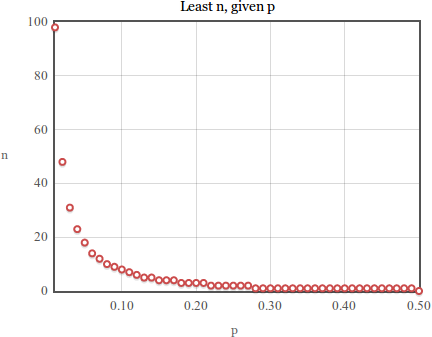
\includegraphics[width=0.45\textwidth]{../graphs/images/restriction-least-n.png}}
  \quad
  \subfloat[Range of possible $p$, given a fixed $n$]{\label{fig:sn-restriction-p-range}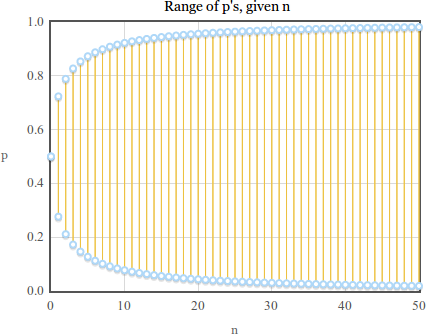
\includegraphics[width=0.45\textwidth]{../graphs/images/restriction-p-range.png}}
  \caption{Restrictions on $n$ and $p$ for estimating $\lambda$}
  \label{fig:sn-restriction}
\end{figure}

It is also possible to fix $n$ and solve for $p$. We return to
\eqref{eq:solving-the-restriction} for further factoring

\begin{align}
  np - np^2 &\geq 1 - 4p + 4p^2 \nonumber \\
  1 - 4p + 4p^2 - np + np^2 &\leq 0 \nonumber \\
  (n+4)p^2 - (n+4)p + 1 &\leq 0 \label{eq: solving for p}
\end{align}

and apply the quadratic formula with $a = n+4$, $b = -(n+4)$, and $c = 1$:

\begin{gather*}
  \frac{(n+4) \pm \sqrt{(n+4)^2 - 4 \cdot (n+4) \cdot 1}}{2(n+4)} \\
  \frac{(n+4) \pm \sqrt{n^2 + 8n + 16 - 4n - 16}}{2(n+4)} \\
  \frac{(n+4) \pm \sqrt{n^2 + 4n}}{2(n-4)} \\
  \frac{n+4}{2(n+4)} \pm \frac12 \sqrt{\frac{n(n+4)}{(n+4)^2}} \\
  \frac12 \pm \frac12 \sqrt{\frac{n}{n+4}}
\end{gather*}

Let $r_1 = \frac12 - \frac12 \sqrt{\frac{n}{n+4}}$ and $r_2 = \frac12 + \frac12
\sqrt{\frac{n}{n+4}}$. (Note that $r_1 < r_2$.) Now we can rewrite \eqref{eq:
solving for p} as

\begin{equation*}
  (p - r_1)(p - r_2) \leq 0
\end{equation*}

Examining the left hand side, when $p < r_1$, both terms are negative and so
their product is positive; when $p > r_2$, both terms are positive, again
leading the product to be positive. Therefore, our solution lies where $r_1
\leq p \leq r_2$, or more explicitly:

\begin{equation}
 \frac12 - \frac12 \sqrt{\frac{n}{n+4}} \; \leq \; p \; \leq \; \frac12 + \frac12 \sqrt{\frac{n}{n+4}}
\end{equation}

As shown in figure \ref{fig:sn-restriction-p-range}, this interval grows
quickly as $n$ increases, and for sufficiently large $n$, it becomes almost
$(0, 1)$. For example, when $n=100$, our interval is $(0.00971, 0.99029)$; when
$n=500$, it is (0.00199, 0.99801).

For $p$ so close to 0 or 1 that this solution will not work, our authors
suggest a Poission approximation.
